\chapter{Aufbau des Gesamtsystems und der Infrastruktur}
In der Endvorstellung des Projektes navigieren vier Roboter simultan durch denselben Raum, woran recht leicht ersichtlich wird, dass ein Weg zum Datenaustausch zwischen den Robotern geschaffen werden muss. Auch eine zentrale Steuereinheit soll in der Lage sein, alle Roboter anzusprechen und zu dirigieren. Selbst ein einzelner Roboter stellt bereits einige Anforderungen an die Kommunikationsstruktur: Da eine erfolgreiche Navigation auf dem Zusammenspiel mehrerer komplexer Algorithmen basiert, müssen externe Analysetools relevante Daten abgreifen, die zwischen den Komponenten ausgetauscht werden. Diese Form des Debuggings ist unerlässlich, um das Verhalten des Roboters nachvollziehen zu können. In diesem Projekt erfüllt ROS diese Anforderungen, weshalb in den folgenden Abschnitten das Kommunikationskonzept unter ROS erläutert wird. Auch die Simulations- und Analysewerkzeuge, die in der Arbeit zum Einsatz kommen, werden vorgestellt und deren ROS-Schnittstellen erläutert.

\begin{figure}[!ht]
\centering
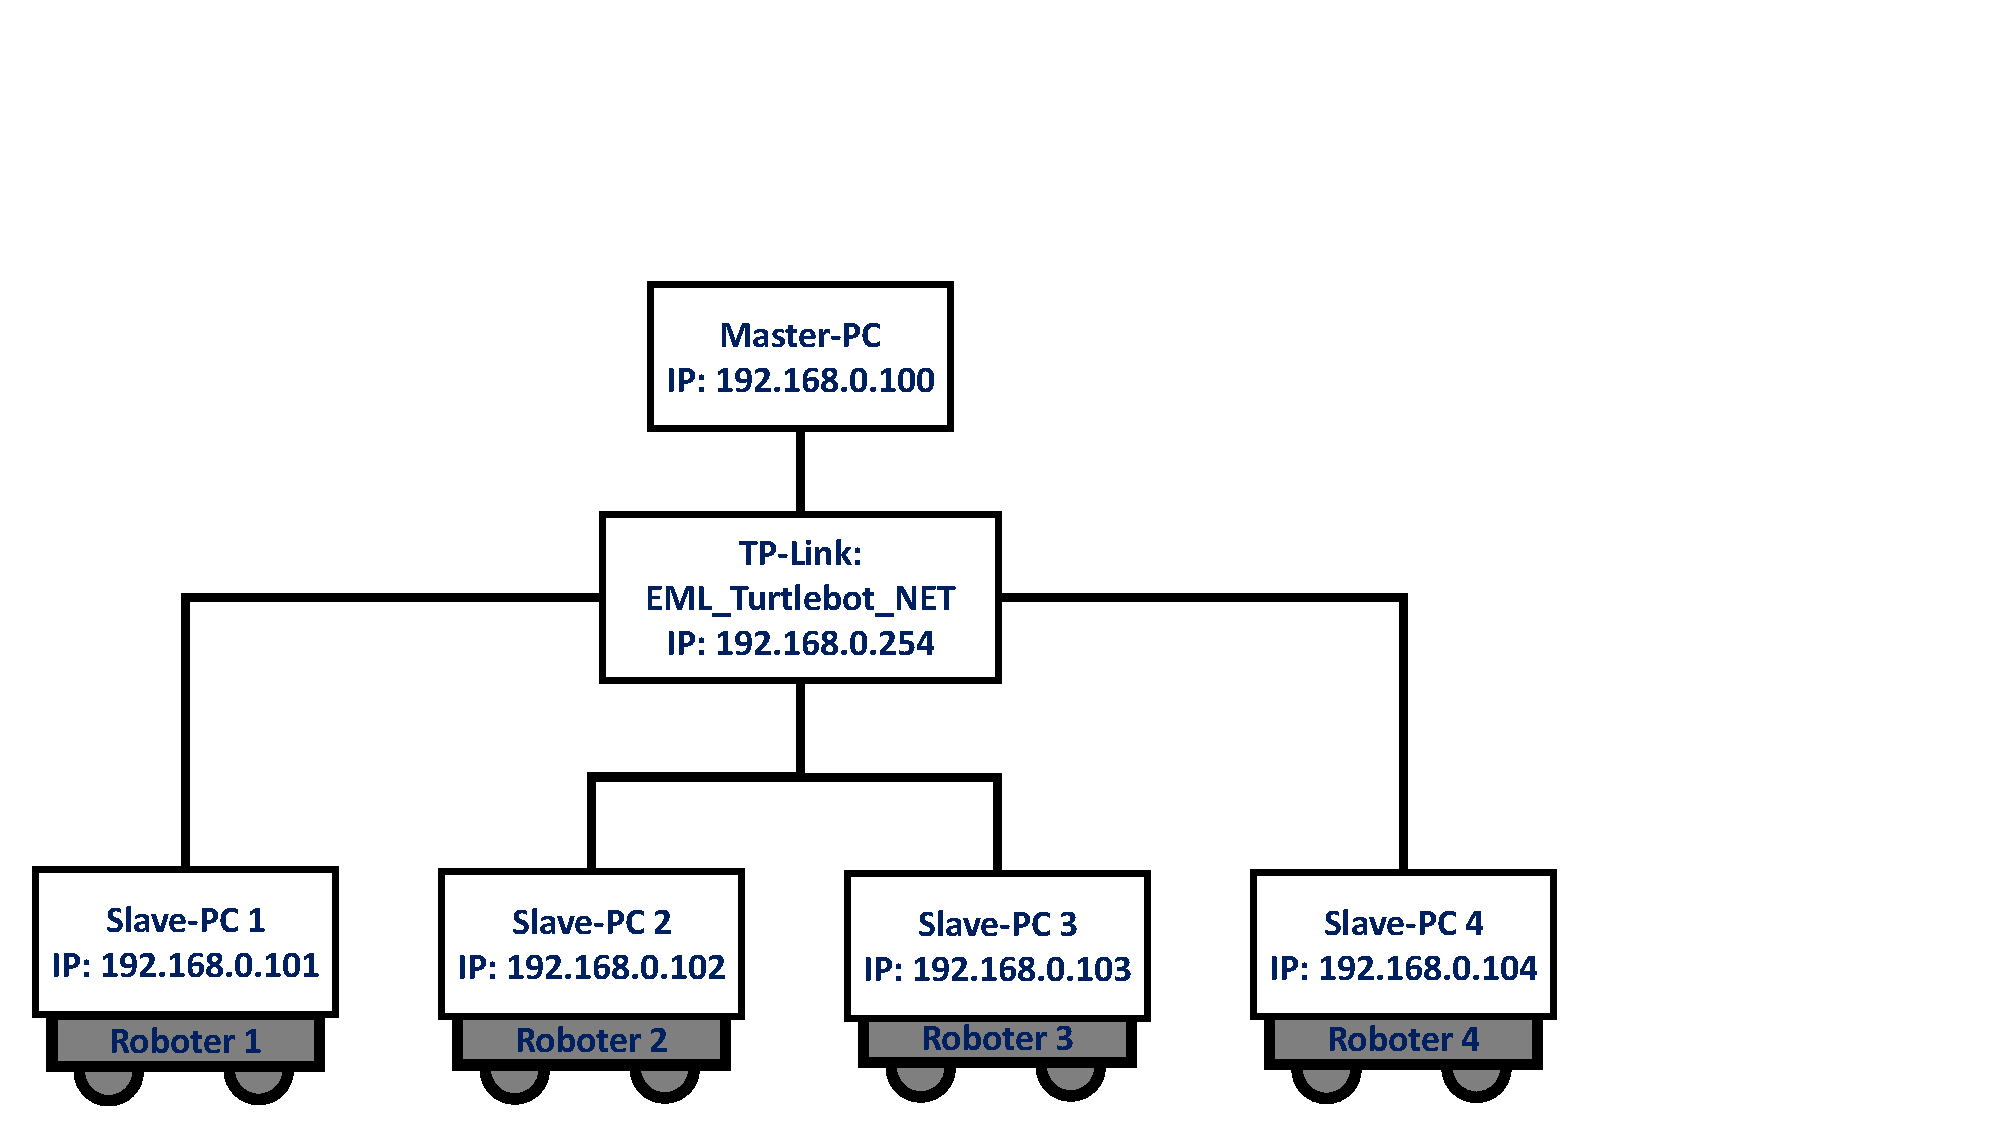
\includegraphics[width=0.9\linewidth, trim={0cm 0cm 6cm 4cm}, clip]{img/Uebersicht_Gesamtsystem.pdf}
\caption{Überblick des Gesamtsystems}
\end{figure}

Jeder TurtleBot ist mit einem Mini-PC ausgestattet, auf denen Ubuntu 14.04 und ROS-Indigo installiert sind. Als zentrale Steuereinheit des Roboterverbundes fungiert ein weiterer Mini-PC, der über WLAN mit den Roboter-PCs verbunden ist. Das private Netzwerk wird mittels eines TP-Link Routers verwaltet, dem auch weitere Entwicklungsrechner beitreten können. Auf dem Master-PC wird \lstinline{ros_core}{} ausgeführt, über den die Kommunikation abläuft. Als Kommunikationsmittel werden in ROS Nachrichten verwendet, die jeweils unter einer so genannten \lstinline{topic}{} veröffentlicht werden. Beispielsweise versendet der Laserscanner zyklisch eine Nachricht des Typs \lstinline{sensor_msg/laser_scan}{} unter der topic \lstinline{/scan}{}. Alle Nodes, die an den Sensordaten interessiert sind, abonnieren die Topic. Indem Analysewerkzeuge wie MATLAB relevante Topics mithören, können die zugehörigen Daten aufgezeichnet und visualisiert werden. Umgekehrt ist es auch möglich den TurtleBot vollständig durch eine Simulation zu ersetzen. GAZEBO veröffentlicht alle Topics, die für gewöhnlich von dem TurtleBot versendet werden, wodurch dieser ersetzt wird. Die restlichen Bestandteile des Netzwerkes bleiben erhalten, weshalb der Wechsel zwischen Realität und Simulation mühelos abläuft.

Die Idee GAZEBO in Verbindung mit ROS für die Simulation zu verwenden entstammt der Arbeit \cite{ROSGazebo}. Dort wurde unter einer ähnlichen Konfiguration ein P3-DX Roboter verwendet. Der primäre Vorteil dieser Simulationsstruktur besteht darin, dass die Algorithmen und Konfigurationen unverändert von der Simulation auf den Roboter übertragen werden können. GAZEBO bietet auch für die TurtelBots eine vollständige Unterstützung, das heißt es besteht eine frei zugängliche Integration des TurtleBot in GAZEBO. Allerdings existiert keine Implementation des hier verwendeten Laserscanner, Tim551, weshalb die Sensorik nicht exakt abgebildet werden kann. Prinzipiell können die Sensoren eingepflegt werden, was jedoch im Rahmen dieser Arbeit aus zeitlichen Gründen nicht erfolgt ist. Daraus resultiert der Nachteil, dass die Simulation nur beschränkt Schlüsse auf die Realität zulässt. Nichtsdestotrotz ergeben sich zwei wichtige Vorteile: Einerseits können die verschiedenen Konfigurationen des ROS-Navigation-Stack anhand der Simulation erprobt und auf ihre Richtigkeit überprüft werden, bevor sie auf reale Anwendungsfälle übertragen werden. Andererseits können im Rahmen der Simulation die Komponenten des Navigation-Stack vollkommen entkoppelt werden. Beispielsweise hängen die Ergebnisse der Navigationsalgorithmen stark von der Qualität der Lokalisierung ab, weshalb die Planungs- und Lokalisierungsproblematik in einem realen Umfeld nicht getrennt untersucht werden können. In der Simulation können Positionsdaten jedoch unmittelbar abgegriffen und der Navigation zur Verfügung gestellt werden. Insofern stellt GAZEBO ein mächtiges Werkzeug für die schrittweise Inbetriebnahme des Navigation-Stacks dar.

MATLAB kann im Rahmen der Robotics-Toolbox ebenfalls als ROS-Node betrieben werden, wodurch eine Schnittstelle zwischen MATLAB und ROS geschaffen wird. Hier bringt MATLAB den Vorteil mit sich, dass es für die Implementierung von Algorithmen oftmals besser geeignet ist als C++ oder auch Python. Insbesondere die Möglichkeiten im Bereich der Visualisierung von Karten und Plots erweisen sich als mächtige Werkzeuge bei der Implementierung und Erprobung von Algorithmen. Außerdem können simple Anwendungsszenarien, wie sie zum Beispiel im Rahmen der diskreten Planung auftreten, vollständig mit MATLAB simuliert werden.

Als letztes Werkzeug sei an dieser Stelle RViz genannt, das als ROS-Paket vorliegt und für die Visualisierung von Robotikanwendungen konzipiert wurde. Mithilfe von RViz können sowohl Karten als auch Roboter und Pfade graphisch dargestellt werden. Da RViz für die Anwendung mit ROS entwickelt wurde, stehen vollständige Konfiguration für den Einsatz mit der autonomen Navigation zur Verfügung, die Out-of-the-Box genutzt werden können.

\section*{Aufbau des ROS-Navigation-Stack}
Der ROS-Navigation-Stack ist das Ergebnis mehrerer zusammengefügter ROS-Pakete für die autonome Navigation von mobilen Robotern. Das Kernpaket, in dem die Navigation implementiert ist, heißt \lstinline{move_base}{}. Die Kernaufgabe des Navigation-Stack besteht darin, eine Weg zwischen Start- und Zielposition zu planen und abzufahren, wofür auf eine Karte der Umgebung zurückgegriffen wird.

Das Planungskonzept des Navigation-Stack verfolgt einen zweischichtigen Ansatz, wobei zwischen einem globalen und einem lokalen Planer differenziert wird. Im ersten Schritt nutzt der globale Planer die vorliegende Karte, um einen ortsdiskreten Pfad zwischen Start- und Zielposition zu bestimmen. Der nächste Punkt des Pfads wird dem lokalen Planer übergeben, der wiederum Geschwindigkeiten berechnen soll, die den Roboter zu dem lokalen Ziel führen. Bei der lokalen Planung werden neben dem nächsten Punkt des globalen Pfades auch die Karte und aktuelle Sensorwerte beachtet. Dieses Vorgehen erinnert an das menschliche Verhalten. Vor einer Autofahrt planen wir anhand einer Karte die Route zum Ziel, was der Aufgabe des globalen Planers entspricht. Hier handelt es sich um eine ortsdiskrete Darstellung, da einzelne Punkte wie Auf- und Abfahrten zu Autobahnen genügen, um den Weg festzulegen. An diesem Zeitpunkt machen wir uns auch noch keine Gedanken, ob wir die Spur wechseln sollen, um den nächsten LKW zu überholen. Derartige Probleme fallen in den Aufgabenbereich des lokalen Planers. Sobald wir uns auf der Reise befinden, und das nächste lokale Ziel - wie zum Beispiel die kommende Autobahnabfahrt - anstreben, planen wir konkrete Überholmanöver. Dennoch können unerwartete Hindernisse, die sich erst während der Fahrt auftun, unsere globalen Pläne über den Haufen werfen. Beispielsweise ziehen wir im Angesicht eines Staus gerne eine Alternativroute in Erwägung. Diese Form der Planänderung wird im Navigation-Stack realisiert, indem einerseits die globale Planung zyklisch wiederholt wird, andererseits werden dabei auch aktuelle Sensorwerte beachtet. So werden Distanzmessungen in die Karte projiziert und als zusätzliche Hindernisse interpretiert, die vom Pfad möglichst gemieden werden sollen.

Wie am Beispiel der Karte und Sensordaten ersichtlich wird, benötigt der Navigation-Stack weitere Informationen, die ihm von außen zur Verfügung gestellt werden müssen. Diese Aufgaben werden mithilfe von weiteren ROS-Paketen erfüllt. Als erstes sei das Paket \lstinline{map_server}{} genannt, der die im Voraus aufgezeichnete Karte unter der Topic \lstinline{\map}{} veröffentlicht. Daraufhin transformiert das Paket \lstinline{costmap_2d}{} die Umgebungskarte in eine sogenannte Kostenkarte, die jeder Zelle einen mit ihrer Durchquerung verbundenen Aufwand zuordnet. Bei der Transformation können zusätzliche Informationen wie zum Beispiel Sensorwerte beachtet werden, wodurch auch Hindernisse, die nicht auf der Karte verzeichnet sind, die Planung beeinflussen. Innerhalb des Navigation-Stacks wird sowohl für den lokalen als auch den globalen Planer eine separate Kostenkarte generiert.
Als letzte wichtige Zusatzinformation ist die Position des Roboters zu nennen, die über zwei relevante Wege bestimmt werden kann. Der einfachste Vorgehensweise nutzt die Odometriedaten, um die Position des Roboters zu berechnen. Einen elaborierteren Ansatz stellt die AMC-Lokalisierung dar, die stochastische Bewegungs- und Messmodelle nutzt, um anhand bekannter Informationen die Position des Roboters zu schätzen. Diese Lokalisierungsvariante wird in dem ROS-Paket \lstinline{amcl}{} implementiert, das simultan zur Navigation ausgeführt wird.
\begin{figure}[!ht]
\centering
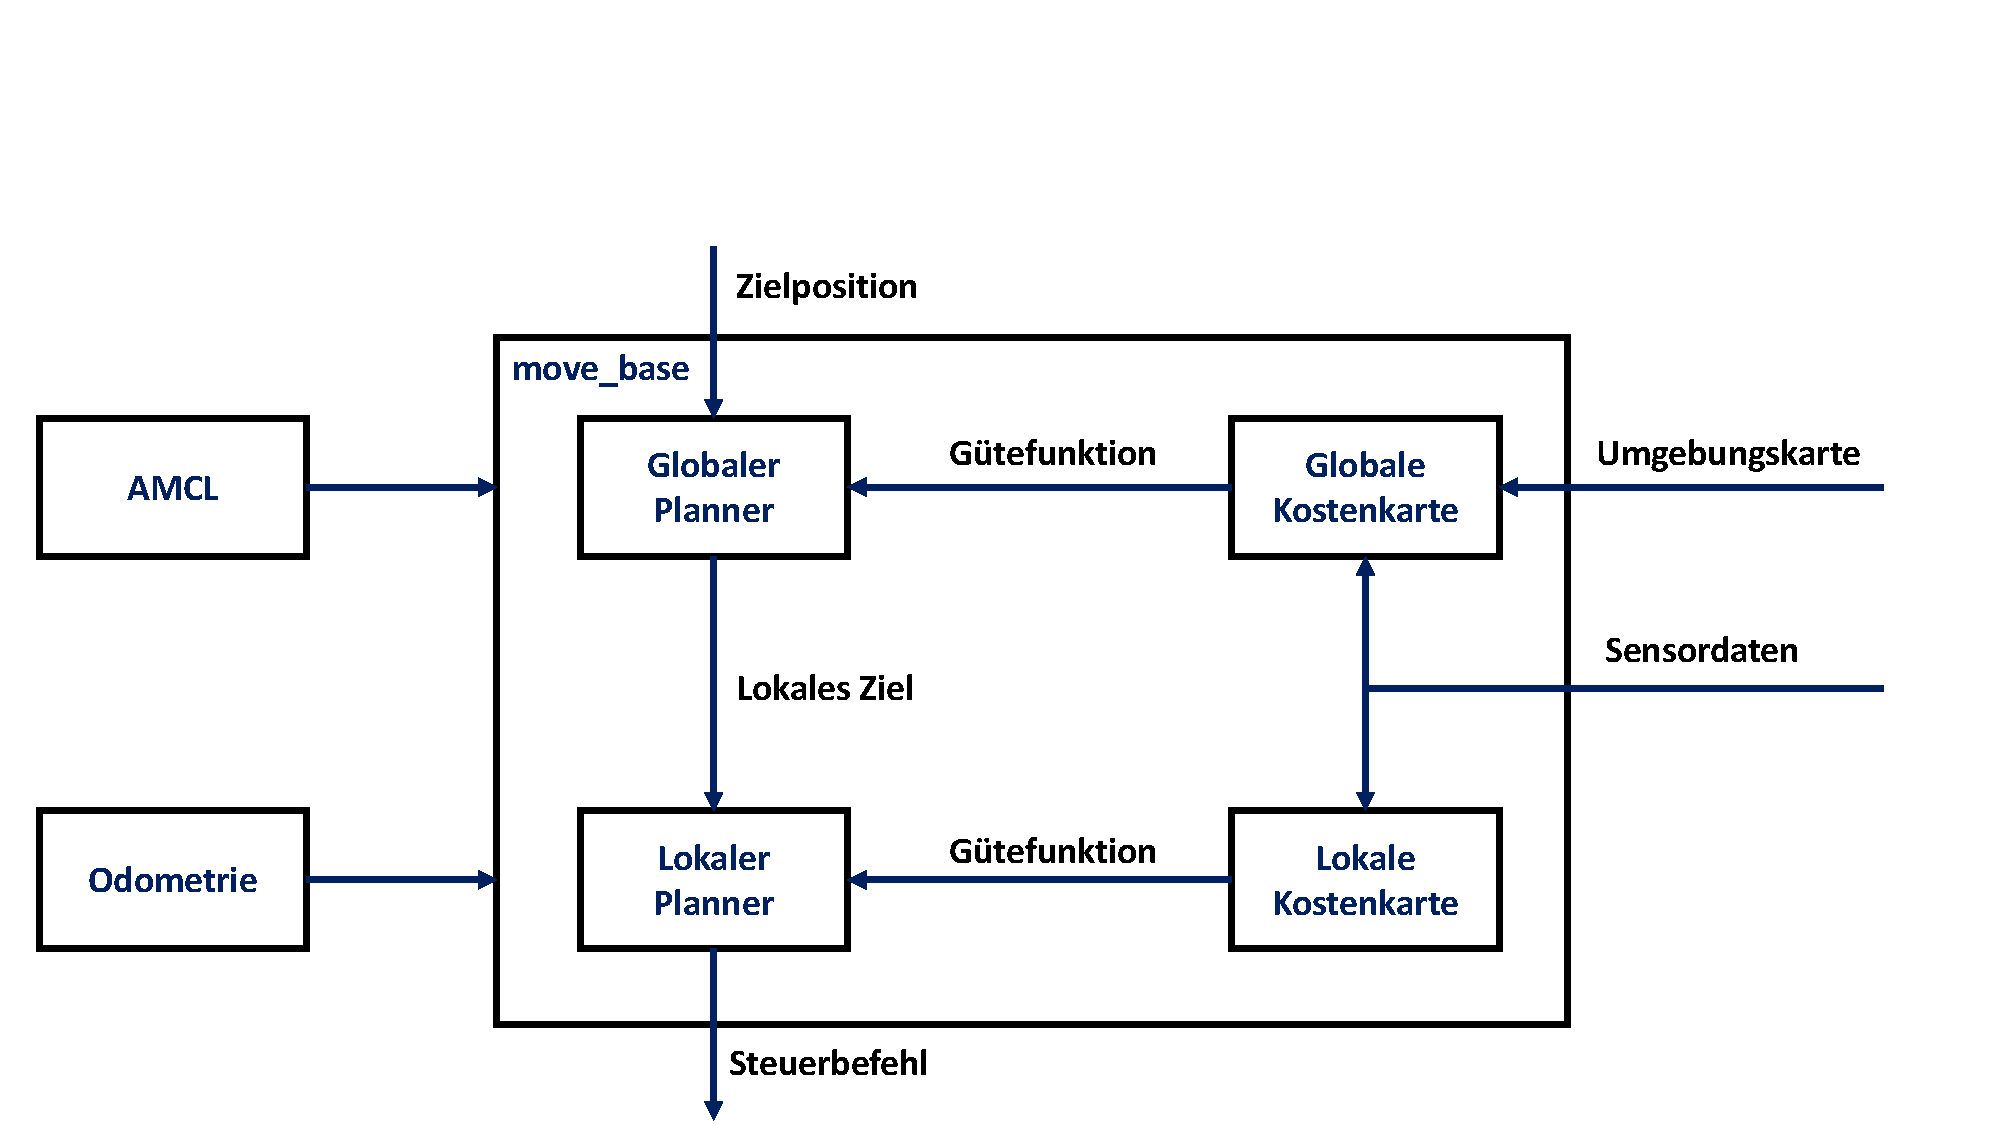
\includegraphics[width=\linewidth,trim={0cm 0cm 2cm 4cm},clip]{img/Navigationstack.pdf}
\caption{Übersicht des Navigationstack, Inhalt teilweise aus \cite{WikiMoveBase}}
\end{figure}

Der nächste Schritt besteht jetzt darin, die einzelnen Teile des Navigation-Stack getrennt zu betrachten und deren zugrundeliegenden Algorithmen zu verstehen. Als erstes wird der globale Planer untersucht, da er einerseits den Ausgangspunkt der Navigation darstellt, andererseits handelt es sich auch um den einzig deterministischen Algorithmus, wodurch er eine Sonderstellung einnimmt. Die restlichen Algorithmen basieren auf stochastischen Konzepten, weshalb anschließend die Rolle der stochastischen Weltanschauung in der Robotik diskutiert wird. Zur Illustration wird sowohl ein stochastisches Bewegungs- als auch Messmodell hergeleitet, die später bei der Lokalisierung und Bewegungsplanung wieder zum Einsatz kommen. Den Ausgangspunkt der meisten Algorithmen stellt das Bayes-Filer dar, das im Folgenden hergeleitet wird und am Beispiel einer simplen Kartographierung illustriert wird. Im nächsten Schritt werden fortgeschrittenere Anwendungen im Rahmen der Lokalisierung betrachtet. Als letzter Bestandteil bleibt der lokale Planer, dessen Dynamic Window Approach zuletzt erläutert wird.